% --- INIZIO NEWCOMMAND ---
% DA METTERE NEL MAIN FILE
\newcommand{\XOR}{\text{\textrm{\color{red}{XOR}}}}

\newcommand*{\circled}[2][red]{
	\tikz[baseline=(char.base)]{
		\node[shape=ellipse,inner sep=2pt,
		draw=#1,
		] (char) {#2};}
}

\newcommand{\markcells}[3][green]{
	\tikz[baseline=(char.mid)]{\node[shape=ellipse,overlay,draw,#1]{\phantom{\rule{#2}{#3}}};}%
}

\newcommand{\negatoA}{\overline{\text{A}}}
\newcommand{\negatoB}{\overline{\text{B}}}
\newcommand{\negatoC}{\overline{\text{C}}}
\newcommand{\negatoD}{\overline{\text{D}}}
\newcommand{\negatoE}{\overline{\text{E}}}

\newcommand{\negatoAbar}{\bar{\text{A}}}
\newcommand{\negatoBbar}{\bar{\text{B}}}
\newcommand{\negatoCbar}{\bar{\text{C}}}
\newcommand{\negatoDbar}{\bar{\text{D}}}
\newcommand{\negatoEbar}{\bar{\text{E}}}

\newcommand{\A}{\text{A}}
\newcommand{\B}{\text{B}}
\newcommand{\C}{\text{C}}
\newcommand{\D}{\text{D}}
\newcommand{\E}{\text{E}}

\newcommand{\distr}{\textrm{\color{red} DISTRIBUTIVE LAW}}
\newcommand{\inverse}{\textrm{\color{red} INVERSE LAW}}
\newcommand{\demorgan}{\textrm{\color{red} DE MORGAN}}
\newcommand{\nulllaw}{\textrm{\color{red} NULL LAW}}
\newcommand{\identity}{\textrm{\color{red} IDENTITY LAW}}
\newcommand{\absorption}{\textrm{\color{red} ABSORPTION LAW}}
\newcommand{\indemp}{\textrm{\color{red} IDEMPOTENT LAW}}

\newcommand{\SOLUZIONE}{\textrm{\textcolor{red}{SOLUZIONE}}}

\newcommand{\logicAND}{\text{{\tiny AND}}}
\newcommand{\logicOR}{\text{{\tiny OR}}}
\newcommand{\logicXOR}{\text{{\tiny XOR}}}

% --- FINE NEWCOMMAND ---

\textsf{\large{\color{red} 6) }} \\

\begin{align*}
	&\text{MOV AX, Mat} \\
	&\text{AND AL, 100b} \\
	&\text{JZ L2} \\
	&\text{OR AH, 1101010b} \\
	&\text{JNZ L3} \\
	&\text{L2: XOR AH, 1010100b} \\
	&\text{L3: MOV Ris6, AX} \\
\end{align*}

\begin{enumerate}
	\item \text{MOV AX, Mat} \\
	\begin{itemize}
		\item \text{AX = 0A2A} \\
	\end{itemize}
	\item \text{AND AL, 100b} \\
		\begin{equation*}
			\begin{tikzpicture}[
				every node/.style={column sep=.5mm,row sep=1mm}]
				\matrix (m) [matrix of math nodes,
				nodes in empty cells,
				%nodes=draw
				] 
				{
					& 0 & 0 & 1 & 0 & 1 & 0 & 1 & 0 & \\    
					& 0 & 0 & 0 & 0 & 0 & 1 & 0 & 0 &[10mm]		\AND\\ 
					& 0 & 0 & 0 & 0 & 0 & 0 & 0 & 0 & \\                                         
				};
				
				\draw[-,color=black,semithick] (m-2-2.south west) -- (m-2-9.south east);
			\end{tikzpicture}
		\end{equation*}
		\textsf{{\small AX = 0A\color{red}00}} \\
		\item \text{JZ L2} \\
		\begin{itemize}
		\item\textsf{{\small JZ sta per "Jump Zero", questo verifica se l'operazione precedente ha dato come risultato 0, se è così \textbf{salta} a L2.}} \\
		\item \textsf{{\small L'operazione precedente si è conclusa con uno zero e quindi passiamo a L2 e saltiamo le operazione che c'erano in mezzo.}} \\
		\end{itemize}
	\item[6.]{L2: XOR AH, 1010100b} \\
		\begin{equation*}
			\begin{tikzpicture}[
				every node/.style={column sep=.5mm,row sep=1mm}]
				\matrix (m) [matrix of math nodes,
				nodes in empty cells,
				%nodes=draw
				] 
				{
					& 0 & 0 & 0 & 0 & 1 & 0 & 1 & 0 & \\    
					& 0 & 1 & 0 & 1 & 0 & 1 & 0 & 0 &[10mm]		\XOR\\ 
					& 0 & 1 & 0 & 1 & 1 & 1 & 1 & 0 & \\                                         
				};
				
				\draw[-,color=black,semithick] (m-2-2.south west) -- (m-2-9.south east);
			\end{tikzpicture}
		\end{equation*}
	\textsf{{\small L'operazione di \textbf{XOR}:}}
	\enlargethispage{42pt}
	\begin{itemize}
		\item \textsf{{\small se i due bit sono diversi il risultato è 1, altrimenti 0.}} \\
	\end{itemize}
	\textsf{{\small AX = \color{red}5E\normalcolor 00}} \\
	\item \text{L3: MOV Ris6, AX} \\
	\text{Ris6 = AX = \color{red}\boxed{\text{\normalcolor 5E00}}} \\
\end{enumerate}

% --- ESERCIZIO 7 ASSEMBLY ---

\pagebreak

\textsf{\large{\color{red} 7) }} \\

\begin{align*}
	&\text{MOV DX, Mat} \\
	&\text{AND DX, 0FF0h} \\
	&\text{CMP DX, 2000} \\
	&\text{JB L4} \\
	&\text{AND DX, 00FFh} \\
	&\text{JMP L5} \\
	&\text{L4: AND DX, 0FF0h} \\
	&\text{L5: LEA ESI, Vet} \\
	&\text{MOV EDI, ESI} \\
	&\text{MOV [EDI], DX} \\
	&\text{INC EDI} \\
	&\text{NOT DX} \\
	&\text{MOV [EDI], DX} \\
	&\text{MOV AX, [ESI]} \\
	&\text{MOV Ris7, AX} \\
\end{align*}

\begin{enumerate}
	\item \text{MOV DX, Mat}
	\textsf{{\small DX = 0A2A}} \\
	\item \text{AND DX, 0FF0h} \\
	\begin{equation*}
		\begin{tikzpicture}[
			every node/.style={column sep=.5mm,row sep=1mm}]
			\matrix (m) [matrix of math nodes,
			nodes in empty cells,
			%nodes=draw
			] 
			{
				& 0 & \text{A} & 2 & \text{A} & \\    
				& 0 & \text{F} & \text{F} & 0 &[10mm]		\AND\\ 
				& 0 & \text{A} & 2 & 0 & \\                                         
			};
			
			\draw[-,color=black,semithick] (m-2-2.south west) -- (m-2-5.south east);
		\end{tikzpicture}
	\end{equation*}
	\item \text{CMP DX, 2000} \\
	\begin{itemize}
		\item \text{DX = 2592 > 2000} \\
	\end{itemize}
	\item \text{JB L4} \\
	\begin{itemize}
		\item \textsf{{\small \textbf{JB} sta per "Jump Below" se è minore, in questo caso, di 2000, ma non è così perchè è maggiore, quindi questo passaggio viene ignorato.}} \\
	\end{itemize}
	\pagebreak
	\item \text{AND DX, 00FFh} \\
	\begin{equation*}
		\begin{tikzpicture}[
			every node/.style={column sep=.5mm,row sep=1mm}]
			\matrix (m) [matrix of math nodes,
			nodes in empty cells,
			%nodes=draw
			] 
			{
				& 0 & \text{A} & 2 & 0 & \\    
				& 0 & 0 & \text{F} & \text{F} &[10mm]		\AND\\ 
				& 0 & 0 & 2 & 0 & \\                                         
			};
			
			\draw[-,color=black,semithick] (m-2-2.south west) -- (m-2-5.south east);
		\end{tikzpicture}
	\end{equation*}
	\item \text{JMP L5} \\
	\begin{itemize}
		\item \textsf{{\small \textbf{JMP} è un salto incodizionato (senza condizioni), salti e basta.}} \\
	\end{itemize}
	\item[8.] \text{L5: LEA ESI, Vet} \\
	\begin{itemize}
		\item \text{ESI = \&Vet} \\
	\end{itemize}
	\item[9.] \text{MOV EDI, ESI} \\
	\begin{itemize}
		\item \text{EDI = ESI = \&Vet} \\
	\end{itemize}
	\item[10.] \text{MOV [EDI], DX} \\
		\begin{tikzpicture}[
			node distance=0pt,
			start chain = A going right,
			X/.style = {rectangle, draw,% styles of nodes in string (chain)
				minimum width=2ex, minimum height=3ex,
				outer sep=0pt, on chain},
			B/.style = {decorate,
				decoration={brace, amplitude=5pt,
					pre=moveto,pre length=1pt,post=moveto,post length=1pt,
					raise=1mm,
					#1}, % for mirroring of brace, if necessary
				thick},
			B/.default=mirror, % by default braces are mirrored
			]
			\foreach \i in {20,00,,,,,,,,,,,,,,,,,,,,,,,,,}% <-- content of nodes
			\node[X] {\i};
			\draw[B] ( A-1.south west) -- node[below=2mm] {MOV [EDI], DX \hspace{0.2cm}\color{red}LITTLE ENDIAN} ( A-2.south east);
			%\draw[B] (A-10.south west) -- node[below=2mm] {Channel 2 Links} (A-18.south east);
			%\draw[B] (A-19.south west) -- node[below=2mm] {Channel 3 Links} (A-27.south east);
			%\node (B1) [inner sep=1pt,above=of A-10.north west] {$\times$};
			%\node (B2) [inner sep=1pt,above=of A-19.north west] {$\times$};
			%\draw[B=](B1.north) -- node[above=2mm] {Crossover Points}(B2.north);
		\end{tikzpicture}
		\item[11.] \text{INC EDI} \\
		\begin{itemize}
			\item \text{EDI = \&(Vet + 1)} \\
		\end{itemize}
	\item[12.] \text{NOT DX} \\
	\begin{itemize}
		\item \textsf{{\small Il \textbf{NOT} nega i valori (ovvero inverte i bits, quelli che sono a 0 diventano 1 e viceversa.) mentre il NEG = registro - 1.}} \\
		\text{DX = $0020_{16} = 0\hspace{.1cm}0\hspace{.1cm}0\hspace{.1cm}0\hspace{.1cm}0\hspace{.1cm}0\hspace{.1cm}0\hspace{.1cm}0\hspace{.1cm}0\hspace{.1cm}0\hspace{.1cm}1\hspace{.1cm}0\hspace{.1cm}0\hspace{.1cm}0\hspace{.1cm}0\hspace{.1cm}0$} \\
		$ \underbrace{1\hspace{.1cm}1\hspace{.1cm}1\hspace{.1cm}1} _{\text{F}} \underbrace{\hspace{.1cm}1\hspace{.1cm}1\hspace{.1cm}1\hspace{.1cm}1} _{\text{F}} \underbrace{\hspace{.1cm}1\hspace{.1cm}1\hspace{.1cm}0\hspace{.1cm}1} _{\text{D}} \underbrace{\hspace{.1cm}1\hspace{.1cm}1\hspace{.1cm}1\hspace{.1cm}1} _{\text{F}} \hspace{.3cm}\textbf{NEGATO} $ \\
		\item\text{DX = FFDF} \\
	\end{itemize}
	\item[13.] \text{MOV [EDI], DX} \\
	\begin{tikzpicture}[
		node distance=0pt,
		start chain = A going right,
		X/.style = {rectangle, draw,% styles of nodes in string (chain)
			minimum width=2ex, minimum height=3ex,
			outer sep=0pt, on chain},
		B/.style = {decorate,
			decoration={brace, amplitude=5pt,
				pre=moveto,pre length=1pt,post=moveto,post length=1pt,
				raise=1mm,
				#1}, % for mirroring of brace, if necessary
			thick},
		B/.default=mirror, % by default braces are mirrored
		]
		\foreach \i in {20,DF,FF,,,,,,,,,,,,,,,,,,,,,,,,}% <-- content of nodes
		\node[X] {\i};
		%\draw[B] ( A-1.south west) -- node[below=2mm] {} ( A-2.south east);
		%\draw[B] (A-10.south west) -- node[below=2mm] {Channel 2 Links} (A-18.south east);
		%\draw[B] (A-19.south west) -- node[below=2mm] {Channel 3 Links} (A-27.south east);
		%\node (B1) [inner sep=1pt,above=of A-10.north west] {$\times$};
		%\node (B2) [inner sep=1pt,above=of A-19.north west] {$\times$};
		%\draw[B=](B1.north) -- node[above=2mm] {Crossover Points}(B2.north);
	\end{tikzpicture} \\
	\textsf{{\small EDI puntava al byte di posizione 1, perchè avevamo fatto l'incremento.}} \\
	\item[14.] \text{AX = DF20} \\
	\enlargethispage{78pt}
	\begin{itemize}
		\item \textsf{{\small EDI puntava alla cella del byte in posizione 0 (ovvero dove si trova 20)}} \\
		\item \textsf{{\small Per via del \textbf{little endian} prendiamo prima il byte che sta dopo ed è per questo che AX equivale a:}} \\
		\item \text{AX = DF20} \\
	\end{itemize}
	%\pagebreak
	\item[15.] \text{MOV Ris7, AX} \\
	\begin{itemize}
		\item \text{Ris7 = AX = \color{red}\boxed{\text{\normalcolor DF20}}} \\
	\end{itemize}
\end{enumerate}

% --- ESERCIZIO 8 ASSEMBLY ---

\newpage

\textsf{\large{\color{red} 8) }} \\

\begin{align*}
	&\text{MOV AX, Mat} \\
	&\text{MOV BL, 5} \\
	&\text{SHL AX, 1} \\
	&\text{JC L6} \\
	&\text{INC BL} \\
	&\text{L6: MUL BL} \\
	&\text{MOV Ris8, AX} \\
\end{align*}

\begin{enumerate}
	\item \text{MOV AX, Mat} \\
	\begin{itemize}
		\item \text{AX = 0A2A} \\
	\end{itemize}
	\item \text{MOV BL, 5} \\
	\begin{itemize}
		\item \text{BL =   5} \\
	\end{itemize}
	\item \text{SHL AX, 1} \\
	\color{red}\sout{\normalcolor 0}\normalcolor $\underbrace{\hspace{.1cm}0\hspace{.1cm}0\hspace{.1cm}0\hspace{.1cm}1} _{1} \underbrace{\hspace{.1cm}0\hspace{.1cm}1\hspace{.1cm}0\hspace{.1cm}0} _{4} \underbrace{\hspace{.1cm}0\hspace{.1cm}1\hspace{.1cm}0\hspace{.1cm}1} _{5}  \underbrace{\hspace{.1cm}0\hspace{.1cm}1\hspace{.1cm}0\hspace{.1cm}\color{red}0}_{\normalcolor 4}$ \\
	\textsf{{\small Il primo 0 va in CF (carry)}} \\
	\item \text{JC L6} \\
	\begin{itemize}
		\item \textsf{{\small \textbf{JC} sta per "Jump Carry" e riguarda il flag del Carry.}} \\
	\end{itemize}
	\item \text{INC BL} \\
	\begin{itemize}
		\item \text{BL = 5 + 1 = 6} \\
	\end{itemize}
	\item \text{MUL BL} \\
	\begin{itemize}
		\item \text{AL = $54_{16} = 01010100_2 = 2^2 + 2^4 + 2^6 = 4 + 16 + 64 = 84_{10} $} \\
		$ 84 \cdot 6 = 504 = 111111000_2 $ \\
		\text{AX = } $ \underbrace{\hspace{.1cm}0\hspace{.1cm}0\hspace{.1cm}0\hspace{.1cm}0} _{0} \underbrace{\hspace{.1cm}0\hspace{.1cm}0\hspace{.1cm}0\hspace{.1cm}1} _{1} \underbrace{\hspace{.1cm}1\hspace{.1cm}1\hspace{.1cm}1\hspace{.1cm}1} _{\text{F}} \underbrace{\hspace{.1cm}1\hspace{.1cm}0\hspace{.1cm}0\hspace{.1cm}0} _{8} $
	\end{itemize}
	\item \text{MOV Ris8, AX} \\
	\begin{itemize}
		\item \text{Ris8 = AX = \color{red}\boxed{\text{\normalcolor 01F8}}} \\
	\end{itemize}
\end{enumerate}

% --- ESERCIZIO 2 ESAME VECCHIO ASSEMBLY ---

\newpage

\textsf{\large{\color{red} 2) Vecchio Esame }} \\

\begin{align*}
	&\text{MOV AX, Mat} \\
	&\text{LEA ESI, Vet} \\
	&\text{ADD ESI, 5} \\
	&\text{MOV ECX, 4} \\
	&\text{L1: MOV [ESI + ECX $\cdot$ 2], AX} \\
	&\text{LOOP L1} \\
	&\text{LEA ESI, Vet} \\
	&\text{ADD ESI, 9} \\
	&\text{MOV DX, [ESI]} \\
	&\text{SHR DX, 4} \\
	&\text{MOV Ris2, DX} \\
\end{align*}

\begin{enumerate}
	\item \text{MOV AX, Mat} \\
	\begin{itemize}
		\item \text{AX = 0A2A} \\
	\end{itemize}
	\item \text{LEA ESI, Vet} \\
	\begin{itemize}
		\item \text{ESI = \&Vet} \\
	\end{itemize}
	\item \text{ADD ESI, 5} \\
	\begin{itemize}
		\item \text{ESI = (\&Vet) + 5} \\
	\end{itemize}
	\item \text{MOV ECX, 4} \\
	\begin{itemize}
		\item \text{ECX =   4} \\
	\end{itemize}
	\item \text{L1: MOV [ESI + ECX $\cdot$ 2], AX} \\
	\item \text{LOOP L1} \\
	\begin{itemize}
		\item \text{ECX = 4 ... ECX = 3 ... ECX = 0 (a 0 ci fermiamo)} \\
	\end{itemize}
	\item \text{LEA ESI,Vet} \\
	\begin{itemize}
		\item \text{ESI = \&Vet}
	\end{itemize}
	\item \text{ADD ESI, 9} \\
	\begin{tikzpicture}[
		node distance=0pt,
		start chain = A going right,
		X/.style = {rectangle, draw,% styles of nodes in string (chain)
			minimum width=2ex, minimum height=3ex,
			outer sep=0pt, on chain},
		B/.style = {decorate,
			decoration={brace, amplitude=5pt,
				pre=moveto,pre length=1pt,post=moveto,post length=1pt,
				raise=1mm,
				#1}, % for mirroring of brace, if necessary
			thick},
		B/.default=mirror, % by default braces are mirrored
		]
		\foreach \i in {,,,,,,2A,0A,2A,0A,2A,0A,2A,0A,,,,,,,,,,,,,}% <-- content of nodes
		\node[X] {\i};
		\draw[B] ( A-9.south west) -- node[below=2mm] {ESI = (\&Vet) + 9} ( A-9.south east);
		%\draw[B] (A-10.south west) -- node[below=2mm] {Channel 2 Links} (A-18.south east);
		%\draw[B] (A-19.south west) -- node[below=2mm] {Channel 3 Links} (A-27.south east);
		%\node (B1) [inner sep=1pt,above=of A-10.north west] {$\times$};
		%\node (B2) [inner sep=1pt,above=of A-19.north west] {$\times$};
		%\draw[B=](B1.north) -- node[above=2mm] {Crossover Points}(B2.north);
	\end{tikzpicture} \\
	\item \text{MOV DX, [ESI]} \\
	\begin{itemize}
		\item \text{DX = 0A2A} \\
	\end{itemize}
	\item \text{SHR DX, 4} \\
	\begin{itemize}
		\item \text{DX = 00A2} \\
	\end{itemize}
	\item \text{MOV Ris2, DX} \\
	\begin{itemize}
		\item \text{Ris2 = DX = \color{red}\boxed{\text{\normalcolor 00A2}}} \\
	\end{itemize}
\end{enumerate}

% --- ALGEBRA DI BOOLE/ PORTE LOGICHE ---
% potrei anche scriverla in un altro file.
\newpage

\section{Algebra di Boole}

% --- ESERCIZIO 1 ALGEBRA DI BOOLE ---

\begin{figure}[ht]
	%\centering
	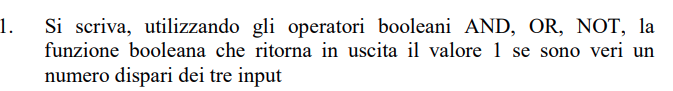
\includegraphics[width=1\linewidth]{es1_pag10_AlgebraDiBoole}
	%\caption{}
	\label{fig:es1pag10algebradiboole}
\end{figure}

\begin{tabular}{|c|c|c||c||c|}
	\hline
	A & B & C & f(a,b,c) & \\
	\hline
	0 & 0 & 0 & 0 & \\
	\hline
	%\rowcolor{BrickRed}
	\tikzmark{starta}0 & 0 & 1 & 1 \tikzmark{enda}& $\bar{\text{A}}\overline{\text{B}}\text{C}$  \\
	\hline
	\tikzmark{startb}0 & 1 & 0 & 1 \tikzmark{endb}& $\overline{\text{A}}\text{B}\overline{\text{C}}$ \\
	\hline
	0 & 1 & 1 & 0 & \\
	\hline
	\tikzmark{startc}1 & 0 & 0 & 1 \tikzmark{endc}& $\text{A}\overline{\text{B}}\overline{\text{C}}$ \\
	\hline
	1 & 0 & 1 & 0 & \\
	\hline
	1 & 1 & 0 & 0 & \\
	\hline
	\tikzmark{startd}1 & 1 & 1 & 1 \tikzmark{endd}& \text{ABC} \\
	\hline  
\end{tabular}

%\markcells{20mm}{1em}
% 	{\circled{\textbf{$M_J=1$}}}& $\textbf{$M_J=2$}$  \\ 
%\begin{comment}
\begin{tikzpicture}[remember picture,overlay]
\foreach \Val in {a, b, c, d}
{
\draw[rounded corners,red,thick]
([shift={(-0.5\tabcolsep,-0.5ex)}]pic cs:start\Val) 
rectangle 
([shift={(0.5\tabcolsep,2ex)}]pic cs:end\Val);
}
\end{tikzpicture}
%\end{comment}

% BUG: PER VIA DEI TIKZMARKS, DA FIXARE.
% BUG FIXATO: Non dare lo stesso nome alle cose in tikzmark e nella tikzpicture.

\begin{comment}

\begin{tikzpicture}[overlay]
	\draw[red, line width=1.5pt] (1,0.3) ellipse (1cm and 0.2cm);
	\draw[blue] (0.35,0.5) ellipse (0.2cm and 0.5cm);
\end{tikzpicture} 

\end{comment}

$ f(\text{A,B,C}) = \bar{\text{A}}\overline{\text{B}}\text{C} + \overline{\text{A}}\text{B}\overline{\text{C}} + \text{A}\overline{\text{B}}\overline{\text{C}} + \text{ABC}  \hspace{0.5cm}\textrm{\color{red} SOLUZIONE}$ \\

\textsf{{\small Il \textbf{+} è considerato un \textbf{OR}. La \textbf{moltiplicazione} è considerata un \textbf{AND}. }} \\

% --- ESERCIZIO 2 ALGEBRA DI BOOLE ---

\begin{figure}[ht]
	%\centering
	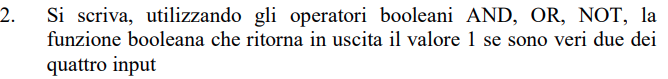
\includegraphics[width=1\linewidth]{es2_pag10_AlgebraDiBoole}
	%\caption{}
	\label{fig:es2pag10algebradiboole}
\end{figure}

\begin{tabular}{|c|c|c|c||c||c|}
	\hline
	A & B & C & D & F & \\
	\hline
	0 & 0 & 0 & 0 & 0 & \\
	\hline
	0 & 0 & 0 & 1 & 0 & \\
	\hline
	0 & 0 & 1 & 0 & 0 & \\
	\hline
	\tikzmark{starte}0 & 0 & 1 & 1 & 1 \tikzmark{ende}& $ \bar{\text{A}}\overline{\text{B}}\text{C}\text{D} $\\
	\hline
	0 & 1 & 0 & 0 & 0 & \\
	\hline
	\tikzmark{startf}0 & 1 & 0 & 1 & 1 \tikzmark{endf}& $ \overline{\text{A}}\text{B}\overline{\text{C}}\text{D} $\\
	\hline
	\tikzmark{startg}0 & 1 & 1 & 0 & 1 \tikzmark{endg}& $ \overline{\text{A}}\text{B}\text{C}\overline{\text{D}} $\\
	\hline
	0 & 1 & 1 & 1 & 0 & \\
	\hline
	1 & 0 & 0 & 0 & 0 & \\
	\hline
	\tikzmark{starth}1 & 0 & 0 & 1 & 1 \tikzmark{endh}& $ \text{A}\bar{\text{B}}\bar{\text{C}}\text{D} $ \\
	\hline
	\tikzmark{starti}1 & 0 & 1 & 0 & 1 \tikzmark{endi}& $ \text{A}\overline{\text{B}}\text{C}\overline{\text{D}} $\\
	\hline
	1 & 0 & 1 & 1 & 0 & \\
	\hline
	\tikzmark{startl}1 & 1 & 0 & 0 & 1 \tikzmark{endl}& $ \text{AB}\bar{\text{C}}\bar{\text{D}} $ \\
	\hline
	1 & 1 & 0 & 1 & 0 & \\
	\hline
	1 & 1 & 1 & 0 & 0 & \\
	\hline
	1 & 1 & 1 & 1 & 0 & \\
	\hline
\end{tabular}
%\begin{comment}
\begin{tikzpicture}[remember picture,overlay]
	\foreach \Val in {e, f, g, h, i, l}
	{
		\draw[rounded corners,red,thick]
		([shift={(-0.5\tabcolsep,-0.5ex)}]pic cs:start\Val) 
		rectangle 
		([shift={(0.5\tabcolsep,2ex)}]pic cs:end\Val);
	}
\end{tikzpicture}
%\end{comment}
\enlargethispage{90pt}
$ f(\text{A,B,C,D}) = \bar{\text{A}}\overline{\text{B}}\text{C}\text{D} + \overline{\text{A}}\text{B}\overline{\text{C}}\text{D} + \overline{\text{A}}\text{B}\text{C}\overline{\text{D}} + \text{A}\bar{\text{B}}\bar{\text{C}}\text{D} + \text{A}\overline{\text{B}}\text{C}\overline{\text{D}} + \text{AB}\bar{\text{C}}\bar{\text{D}} \hspace{0.5cm}\textrm{\color{red} SOLUZIONE}$ \\

% --- ESERCIZIO 3 ALGEBRA DI BOOLE ---

\newpage

\begin{figure}[ht]
	%\centering
	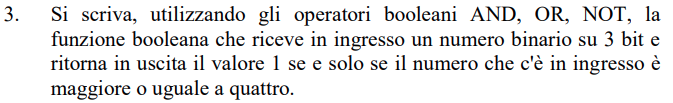
\includegraphics[width=1\linewidth]{es3_pag10_AlgebraDiBoole}
	%\caption{}
	\label{fig:es3pag10algebradiboole}
\end{figure}

\textsf{{\small 3 variabili (A,B,C) e quindi 8 combinazioni}} \\
\begin{itemize}
	\item \textsf{{\small Nella prima a destra (la C) ripetizioni 0 1 (in verticale)}} \\
	\item \textsf{{\small Nella centrale (la B) ripetizione: 0 0 1 1 (in verticale)}} \\
	\item \textsf{{\small In quella a sinistra (la A) ripetizioni 0 0 0 0 1 1 1 1}} \\
\end{itemize}

\begin{tabular}{|c|c|c||c||c|}
	\hline
	A & B & C & f(a,b,c) & \\
	\hline
	0 & 0 & 0 & 0 & \\
	\hline
	0 & 0 & 1 & 0 & \\
	\hline
	0 & 1 & 0 & 0 & \\
	\hline
	0 & 1 & 1 & 0 & \\
	\hline
	\tikzmark{startup}1 & 0 & 0 & 1 \tikzmark{endup}& \text{A}$ \bar{\text{B}}\bar{\text{C}} $\\
	\hline
	\tikzmark{startup2}1 & 0 & 1 & 1 \tikzmark{endup2}& \text{A}$ \overline{\text{B}} $ \text{C}\\
	\hline
	\tikzmark{startdown}1 & 1 & 0 & 1 \tikzmark{enddown}& \text{AB}$ \overline{\text{C}} $\\
	\hline
	\tikzmark{startdown2}1 & 1 & 1 & 1 \tikzmark{enddown2}& \text{ABC} \\
	\hline  
\end{tabular}

%\begin{comment}
\begin{tikzpicture}[remember picture,overlay]
	\foreach \Val in {up, up2, down, down2}
	{
		\draw[rounded corners,red,thick]
		([shift={(-0.5\tabcolsep,-0.5ex)}]pic cs:start\Val) 
		rectangle 
		([shift={(0.5\tabcolsep,2ex)}]pic cs:end\Val);
	}
\end{tikzpicture}
%\end{comment}

\begin{tikzpicture}[overlay]
	%\draw[red, line width=1.5pt] (1,0.3) ellipse (1cm and 0.2cm);
	%\draw[blue, line width=.9pt] (0.35,1.6) ellipse (0.2cm and 1.2cm);
	\draw[blue, line width=.9pt] (0.35,2.7) ellipse (0.2cm and 2.2cm);
	\draw[blue, line width=.9pt] (3.1,2.7) ellipse (0.2cm and 2.2cm);
\end{tikzpicture}

$ f(\text{A,B,C}) = \text{A}\bar{\text{B}}\bar{\text{C}} + \text{A}\overline{\text{B}} \text{C} + \text{AB} \overline{\text{C}} + \text{ABC} \hspace{0.5cm} \textrm{\color{red} SOLUZIONE}$ \\

\textsf{{\small La soluzione può anche essere scritta: }} \\

$ f(\text{A,B,C}) = \text{A} $ \\

\textsf{{\small La colonna A è uguale alla colonna di F (non solo quei quattro 1, ma tutta la colonna dall'inizio, zeri compresi), se dovessi solo restituire A è come se restituissi F.}} \\

% --- ESERCIZIO 4 ALGEBRA DI BOOLE ---

\pagebreak

\begin{figure}[ht]
	%\centering
	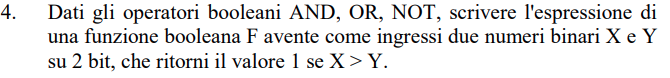
\includegraphics[width=1\linewidth]{es4_pag10_AlgebraDiBoole}
	%\caption{}
	\label{fig:es4pag10algebradiboole}
\end{figure}
%\enlargethispage{320pt}
\begin{tabular}{|c|c|c|c||c||c|c|c|}
	\hline
	$\color{blue}\mathbf{x_1}$ & $\color{blue}\mathbf{x_0}$ & $\color{green}\mathbf{y_1}$ & $\mathbf{\color{green}y_0}$ & $f(x,y)$ & $ \mathbf{\color{blue}x_1 x_0}$& $ \mathbf{\color{green} y_1 y_0} $ &\\
	\hline
	0 & 0 & 0 & 0 & \color{red}0 & \color{blue}0 & \color{green}0 &\\
	\hline
	0 & 0 & 0 & 1 & \color{red}0 & \color{blue}0 & \color{green}1 &\\
	\hline
	0 & 0 & 1 & 0 & \color{red}0 & \color{blue}0 & \color{green}2 &\\
	\hline
	0 & 0 & 1 & 1 & \color{red}0 & \color{blue}0 & \color{green}3 &\\
	\hline
	\tikzmark{startm}0 & 1 & 0 & 0 & \color{red}1\tikzmark{endm} & \color{blue}1 & \color{green}0& $ \mathbf{\overline{x_1}x_0\overline{y_1}\bar{y_0}} $\\
	\hline
	0 & 1 & 0 & 1 & \color{red}0 & \color{blue}1 & \color{green} 1 &\\
	\hline
	0 & 1 & 1 & 0 & \color{red}0 & \color{blue}1 & \color{green} 2 &\\
	\hline
	0 & 1 & 1 & 1 & \color{red}0 & \color{blue}1 & \color{green}3 &\\
	\hline
	\tikzmark{startn}1 & 0 & 0 & 0 & \color{red}1\tikzmark{endn} & \color{blue}2 & \color{green}0 & $ \mathbf{x_1\overline{x_0}\bar{y_1}\overline{y_0}} $\\
	\hline
	\tikzmark{starto}1 & 0 & 0 & 1 & \color{red}1\tikzmark{endo} & \color{blue}2 & \color{green}1 & $ \mathbf{x_1 x_0 \bar{y_1}\overline{y_0}} $ \\
	\hline
	1 & 0 & 1 & 0 & \color{red}0 & \color{blue}2 & \color{green}2 &\\
	\hline
	1 & 0 & 1 & 1 & \color{red}0 & \color{blue}2 & \color{green}3 &\\
	\hline
	\tikzmark{startp}1 & 1 & 0 & 0 & \color{red}1\tikzmark{endp} & \color{blue}3 & \color{green}0 & $ \mathbf{x_1 x_0 \bar{y_1} \overline{y_0}} $\\
	\hline
	\tikzmark{startq}1 & 1 & 0 & 1 & \color{red}1\tikzmark{endq} & \color{blue}3 & \color{green}1 & $ \mathbf{x_1 x_0 \overline{y_1} y_0} $\\
	\hline
	\tikzmark{startr}1 & 1 & 1 & 0 & \color{red}1\tikzmark{endr} & \color{blue}3 & \color{green}2 & $ \mathbf{x_1 x_0 y_1 \overline{y_0}} $\\
	\hline
	1 & 1 & 1 & 1 & \color{red}0 & \color{blue}3 & \color{green}3 &\\
	\hline
\end{tabular}
%\begin{comment}
\begin{tikzpicture}[remember picture,overlay]
\foreach \Val in {m, n, o, p, q, r}
{
\draw[rounded corners,blue,thick]
([shift={(-0.5\tabcolsep,-0.5ex)}]pic cs:start\Val) 
rectangle 
([shift={(0.5\tabcolsep,2ex)}]pic cs:end\Val);
}
\end{tikzpicture}
%\end{comment}

$ f(x,y) = \mathbf{\overline{x_1}x_0\overline{y_1}\bar{y_0}} + \mathbf{x_1\overline{x_0}\bar{y_1}\overline{y_0}} + \mathbf{x_1 x_0 \bar{y_1}\overline{y_0}} + \mathbf{x_1 x_0 \bar{y_1} \overline{y_0}} + \mathbf{x_1 x_0 \overline{y_1} y_0} + \mathbf{x_1 x_0 y_1 \overline{y_0}}$ \\

\textsf{{\small Le colonne: $ \mathbf{\color{blue} x_1 x_0} \text{ e } \mathbf{\color{green}y_1 y_0 }$ sono in decimale considerando due bit.}} \\

% --- TABELLA PROPRITA' FUNZIONI BOOLEANE ---

\subsection{Tabella delle Proprietà delle Funzioni Booleane}

\begin{figure}[ht]
	\centering
	\includegraphics[width=0.7\linewidth]{tabella_proprietà_funzioni_booleane}
	%\caption{Tabella delle Proprietà delle Funzioni Booleane}
	\label{fig:tabella_proprietà_funzioni_booleane}
\end{figure}

% --- ESERCIZIO 5 ALGEBRA DI BOOLE ---

\newpage

\begin{figure}[ht]
	%\centering
	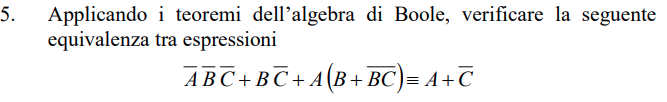
\includegraphics[width=1\linewidth]{es5_pag11_AlgebraDiBoole}
	%\caption{}
	\label{fig:es5pag11algebradiboole}
\end{figure}

\textsf{{\small Cerchiamo di semplificare l'espressione}} \\
 
\begin{equation*}
	\underbrace{\negatoA\negatoBbar\negatoC + \B\negatoC} _{\negatoC(\negatoAbar\negatoB + \B) \hspace{0.3cm}\textrm{\color{red}PROPRIETA' DISTRIBUTIVA}} + 
	\A(\B + \underbrace{\negatoB\negatoC)} 
	_{\A(\B + \negatoB + \negatoC) \hspace{0.3cm}\textrm{\color{red} APPLICHIAMO DE MORGAN}}
\end{equation*}

\begin{equation*}
\negatoC(\underbrace{\negatoAbar\negatoB + \B} _{\negatoC((\negatoA + \B) \cdot (\negatoB + \B)) \textrm{\color{red} \hspace{0.2cm}distr.}}) + \A(\underbrace{\B + \negatoB} _{\A(1 + \negatoC) \hspace{0.2cm}\textrm{\color{red}inverse law}} + \negatoC) 
\end{equation*}

\begin{equation*}
	\C((\negatoA + \B) \cdot (\underbrace{\negatoB + \B} _{\inverse}) ) + \A(\underbrace{1 + \negatoC} _{\nulllaw})
\end{equation*}

\begin{equation*}
	\negatoC(\underbrace{(\negatoA + \B) \cdot 1} _{\identity}) + \underbrace{\A \cdot 1} _{\identity}
\end{equation*}

\begin{equation*}
	\underbrace{\negatoC(\negatoA + \B)} _{\distr} + \A
\end{equation*}

\begin{equation*}
	\underbrace{\negatoC\negatoAbar + \negatoC\B + \A} _{\distr}
\end{equation*}

\begin{equation*}
	(\A + \negatoC)(\underbrace{\A + \negatoA} _{\inverse}) + \negatoC\B
\end{equation*}

\begin{equation*}
	\underbrace{(\A + \negatoC) \cdot 1} _{\identity} + \negatoC\B
\end{equation*}

\begin{equation*}
	(\A + \negatoC) + \negatoC\B
\end{equation*}

\begin{equation*}
\A + \underbrace{\negatoC + \negatoC\B} _{\absorption}
\end{equation*}

\begin{equation*}
	\A + \negatoC
\end{equation*}

% --- ESERCIZIO 6 ---

\pagebreak

\begin{figure}[ht]
	%\centering
	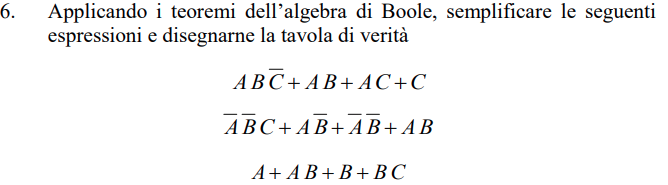
\includegraphics[width=1\linewidth]{es6_pag11_AlgebraDiBoole}
	%\caption{}
	\label{fig:es6pag11algebradiboole}
\end{figure}

\centering
 $\underbrace{\A\B\negatoC + \A\B} _{\absorption} + \underbrace{\A\C + \C} _{\absorption}  $\\
	 $\A\B + \C $ \\
\flushleft

\begin{tabular}{|c|c|c|c||c||c|c|c|}
	\hline
	A & B & C & $\overset{x}{\A\B}$ & $\overset{y}{\A\C}$ & $\overset{z}{AB\negatoC}$ & $ z + x + y + c $ & $x + c$\\
	\hline
	0 & 0 & 0 & 0 & 0 & 0 & 0 & 0\\
	\hline
	0 & 0 & 1 & 0 & 0 & 0 & 1 & 1\\
	\hline
	0 & 1 & 0 & 0 & 0 & 0 & 0 & 0\\
	\hline
	0 & 1 & 1 & 0 & 0 & 0 & 1 & 1\\
	\hline
	1 & 0 & 0 & 0 & 0 & 0 & 0 & 0\\
	\hline
	1 & 0 & 1 & 0 & 1 & 0 & 1 & 1\\
	\hline
	1 & 1 & 0 & 1 & 0 & 1 & 1 & 1\\
	\hline
	1 & 1 & 1 & 1 & 1 & 0 & 1 & 1\\
	\hline
\end{tabular}

\begin{tikzpicture}[overlay]
	%\draw[red, line width=1.5pt] (1,0.3) ellipse (1cm and 0.2cm);
	\draw[red, line width=.9pt] (6.87,2.1) ellipse (0.2cm and 2.2cm);
	\draw[red, line width=.9pt] (8.75,2.1) ellipse (0.2cm and 2.2cm);
	%\draw[blue, line width=.9pt] (3.1,2.7) ellipse (0.2cm and 2.2cm);
\end{tikzpicture}

\textsf{{\small Le due colonne cerchiate in \textcolor{red}{rosso} sono equivalenti.}} \\

\textrm{\color{red} ES.6 - N.2} \\

\centering
$ \underbrace{\negatoA\negatoBbar} _{\absorption} \C + \A\negatoB + \underbrace{\negatoA\negatoBbar} _{\absorption} + \A\B $ \\

$ \negatoA\negatoBbar + \underbrace{\A\negatoB + \A\B} _{\distr} $ \\

$ \negatoA\negatoBbar + \A(\underbrace{\negatoB + \B} _{\inverse}) $ \\

$ \negatoA\negatoBbar + \underbrace{\A \cdot 1} _{\identity} $ \\

$ \underbrace{\negatoA\negatoBbar + \negatoA} _{\distr} $ \\

$ \underbrace{(\A + \negatoA)} _{\inverse}(\A + \negatoB) $ \\

$ \underbrace{1 \cdot(\A + \negatoB)} _{\identity} $ \\

$ \color{red}\boxed{\normalcolor\A + \negatoB} $ \\

\enlargethispage{30pt}
\textsf{{\small Ora non più semplificabile.}} \\

\centering

\pagebreak

\begin{tabular}{|c|c|c|c||c||c|c|c|c|}
	\hline
	A & B & C & $\overset{x}{\negatoA\negatoBbar}$ & $\overset{y}{X\C}$ & $\overset{z}{A\negatoB}$ & $ \overset{t}{\A\B} $ &$ y + z + x + t $ & $\A + \negatoB$\\
	\hline
	0 & 0 & 0 & 1 & 0 & 0 & 0 & 1 & 1\\
	\hline
	0 & 0 & 1 & 1 & 1 & 0 & 0 & 1 & 1\\
	\hline
	0 & 1 & 0 & 0 & 0 & 0 & 0 & 0 & 0\\
	\hline
	0 & 1 & 1 & 0 & 0 & 0 & 0 & 0 & 0\\
	\hline
	1 & 0 & 0 & 0 & 0 & 1 & 0 & 1 & 1\\
	\hline
	1 & 0 & 1 & 0 & 1 & 1 & 0 & 1 & 1\\
	\hline
	1 & 1 & 0 & 0 & 0 & 0 & 1 & 1 & 1\\
	\hline
	1 & 1 & 1 & 0 & 0 & 0 & 1 & 1 & 1\\
	\hline
\end{tabular}

\begin{tikzpicture}[overlay]
	%\draw[red, line width=1.5pt] (1,0.3) ellipse (1cm and 0.2cm);
	\draw[red, line width=.9pt] (2.45,2.1) ellipse (0.2cm and 2.2cm);
	\draw[red, line width=.9pt] (4.42,2.1) ellipse (0.2cm and 2.2cm);
	%\draw[blue, line width=.9pt] (3.1,2.7) ellipse (0.2cm and 2.2cm);
\end{tikzpicture}

\textsf{{\small Le due colonne cerchiate in \textcolor{red}{rosso} sono equivalenti.}} \\

\flushleft

% --- ESERCIZIO 7 ALGEBRA DI BOOLE ---

\begin{figure}[ht]
	%\centering
	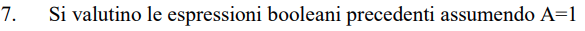
\includegraphics[width=1\linewidth]{es7_pag11_AlgebraDiBoole}
	%\caption{}
	\label{fig:es7pag11algebradiboole}
\end{figure}

\pagebreak

% --- ESERCIZIO 8 ALGEBRA DI BOOLE ---

\begin{figure}[ht]
	%\centering
	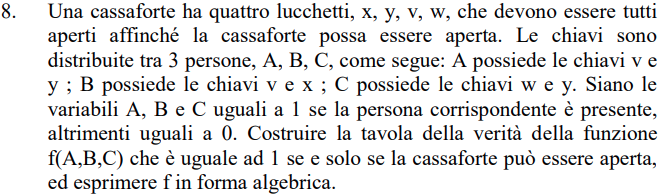
\includegraphics[width=1\linewidth]{es8_pag11_AlgebraDiBoole}
	%\caption{}
	\label{fig:es8pag11algebradiboole}
\end{figure}

\centering

\begin{tabular}{|c|c|c||c||c|}
	\hline
	A & B & C & $f$ & \\
	\hline
	0 & 0 & 0 & 0 & \\
	\hline
	0 & 0 & 1 & 0 & \\
	\hline
	0 & 1 & 0 & 0 & \\
	\hline
	\tikzmark{starts}0 & 1 & 1 & 1 \tikzmark{ends}& $ \negatoA\B\C $\\
	\hline
	1 & 0 & 0 & 0 & \\
	\hline
	1 & 0 & 1 & 0 & \\
	\hline
	1 & 1 & 0 & 0 & \\
	\hline
	\tikzmark{startt}1 & 1 & 1 & 1 \tikzmark{endt}& \A\B\C \\
	\hline  
\end{tabular}

\begin{tikzpicture}[remember picture,overlay]
	\foreach \Val in {s, t}
	{
		\draw[rounded corners,red,thick]
		([shift={(-0.5\tabcolsep,-0.5ex)}]pic cs:start\Val) 
		rectangle 
		([shift={(0.5\tabcolsep,2ex)}]pic cs:end\Val);
	}
\end{tikzpicture}

\centering

$ f(\A, \B, \C) = \underbrace{\negatoA\B\C + \A\B\C} _{\distr} $ \\

$ \B\C\underbrace{(\negatoA + \A)} _{\inverse} $ \\

$ \underbrace{\B\C \cdot 1} _{\identity} $ \\

$ \color{red}\boxed{\normalcolor\B\C} \hspace{0.3cm}\textrm{\color{red} SOLUZIONE}$ \\

% --- NOT OR AND LOGIC GATES ---

\subsection{NOT - OR - AND | LOGIC GATES}

\begin{figure}[ht]
	%\centering
	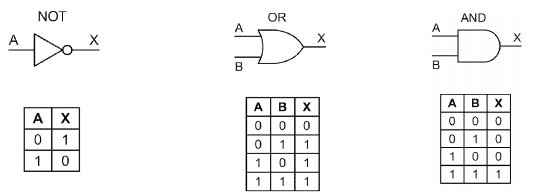
\includegraphics[width=.8\linewidth]{not_or_and_logic_gates}
	%\caption{}
	\label{fig:not_or_and_logic_gates}
\end{figure}

% --- ESERCIZIO 9 ALGEBRA DI BOOLE ---

\newpage

\begin{figure}[ht]
	%\centering
	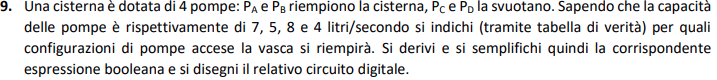
\includegraphics[width=1\linewidth]{es9_esBoole}
	%\caption{}
	\label{fig:es9esBoole}
\end{figure}

%\enlargethispage{120pt}

\begin{tabular}{|c|c|c|c||c||c|}
	\hline
	A & B & C & D & $f$ & \\
	\hline
	0 & 0 & 0 & 0 & 0 & \\
	\hline
	0 & 0 & 0 & 1 & 0 & \\
	\hline
	0 & 0 & 1 & 0 & 0 & \\
	\hline
	0 & 0 & 1 & 1 & 0 & \\
	\hline
	\tikzmark{startu}0 & 1 & 0 & 0 & 1 \tikzmark{endu}& $ \negatoA\B\negatoC\negatoDbar $\\
	\hline
	\tikzmark{startv}0 & 1 & 0 & 1 & 1 \tikzmark{endv}& $ \negatoA\B\negatoC\D $\\
	\hline
	0 & 1 & 1 & 0 & 0 & \\
	\hline
	0 & 1 & 1 & 1 & 0 & \\
	\hline
	\tikzmark{startz}1 & 0 & 0 & 0 & 1 \tikzmark{endz}& $ \A\negatoB\negatoCbar\negatoD $\\
	\hline
	\tikzmark{startw}1 & 0 & 0 & 1 & 1 \tikzmark{endw}& $ \A\negatoB\negatoCbar\D $\\
	\hline
	1 & 0 & 1 & 0 & 0 & \\
	\hline
	1 & 0 & 1 & 1 & 0 & \\
	\hline
	\tikzmark{startj}1 & 1 & 0 & 0 & 1 \tikzmark{endj}& $ \A\B\negatoC\negatoDbar $\\
	\hline
	\tikzmark{starty}1 & 1 & 0 & 1 & 1 \tikzmark{endy}& $ \A\B\negatoC\D $\\
	\hline
	\tikzmark{startx}1 & 1 & 1 & 0 & 1 \tikzmark{endx}& $ \A\B\C\negatoD $\\
	\hline
	1 & 1 & 1 & 1 & 0 & \\
	\hline
\end{tabular}

\begin{tikzpicture}[remember picture,overlay]
	\foreach \Val in {u, v, z, w, j, y, x}
	{
		\draw[rounded corners,red,thick]
		([shift={(-0.5\tabcolsep,-0.5ex)}]pic cs:start\Val) 
		rectangle 
		([shift={(0.5\tabcolsep,2ex)}]pic cs:end\Val);
	}
\end{tikzpicture}

	
$ f(\A, \B, \C, \D) = \negatoA\B\negatoC\negatoDbar + \negatoA\B\negatoC\D + \A\negatoB\negatoCbar\negatoD + \A\negatoB\negatoCbar\D + \A\B\negatoC\negatoDbar + \A\B\negatoC\D + \A\B\C\negatoD $ \break

$ \underbrace{\negatoA\B\negatoC\negatoDbar + \negatoA\B\negatoC\D} _{} + \underbrace{\A\negatoB\negatoCbar\negatoD + \A\negatoB\negatoCbar\D} _{} + \underbrace{\A\B\negatoC\negatoDbar + \A\B\negatoC\D} _{} + \A\B\C\negatoD + \negatoA\B\negatoC(\underbrace{\negatoD + \D} _{\inverse}) + \A\negatoBbar\negatoC(\underbrace{\negatoD + \D} _{\inverse}) + \A\B\negatoC(\underbrace{\negatoD + \D} _{\inverse}) $ \\

$ \Rightarrow \negatoA\B\negatoC + \A\negatoBbar\negatoC + \underbrace{\A\B\negatoC + \A\B\C\negatoD} _{} + \A\B(\underbrace{\negatoC + \C\negatoD} _{\negatoC + \negatoD})$ \\

$ \underbrace{\negatoA\B\negatoC} _{} + \A\negatoBbar\negatoC + \underbrace{\A\B\negatoC} _{} + \A\B\negatoD$ \\

$ \B\negatoC(\underbrace{\negatoA + \A} _{1\inverse}) $ \\

$ \underbrace{\B\negatoC + \A\negatoBbar\negatoC} _{} + \A\B\negatoD + \negatoC(\underbrace{\A + \A\negatoB} _{\B + \A})$ \\

$ \A\negatoC + \underbrace{\B\negatoC + \A\B\negatoD} _{\B(\negatoC + \A\negatoD)} $ \\

$ \color{red}\boxed{\normalcolor\A\negatoC + \B(\negatoC + \A\negatoD)} \hspace{0.3cm}\SOLUZIONE$ \\

\begin{comment}
\begin{circuitikz} \draw
	(0,2) node[and port] (myand1) {}
	(0,0) node[and port] (myand2) {}
	(2,1) node[xnor port] (myxnor) {}
	(myand1.out) -- (myxnor.in 1)
	(myand2.out) -- (myxnor.in 2);
\end{circuitikz}
\end{comment}

\begin{comment}
\begin{tikzpicture}[label distance=2mm]
	
	\node (x3) at (0,0) {\A};
	\node (x2) at (1,0) {\B};
	\node (x1) at (2,0) {\C};
	\node (x0) at (3,0) {\D};
	
	\node (x4) at (0.5, -0.3) {$ \negatoA $};
	\node (x5) at (1.5, -0.3) {$ \negatoB $};
	\node (x6) at (2.5, -0.3) {$ \negatoC $};
	\node (x7) at (3.5, -0.3) {$ \negatoD $};
	
	\node[not gate US, draw, rotate=-90] at ($(x3)+(0.5,-1)$) (Not3) {};
	\node[not gate US, draw, rotate=-90] at ($(x2)+(0.5,-1)$) (Not2) {};
	\node[not gate US, draw, rotate=-90] at ($(x1)+(0.5,-1)$) (Not1) {};
	\node[not gate US, draw, rotate=-90] at ($(x0)+(0.5,-1)$) (Not0) {};
	
	\node[or gate US, draw, logic gate inputs=nnn] at ($(x0)+(2,-2)$) (Or1) {};
	\node[or gate US, draw, logic gate inputs=nnnn] at ($(Or1)+(0,-1)$) (Or2) {};
	\node[or gate US, draw, logic gate inputs=nnn] at ($(Or2)+(0,-1)$) (Or3) {};
	\node[xor gate US, draw, logic gate inputs=nn] at ($(Or3)+(0,-1)$) (Xor1) {};
	\node[and gate US, draw, logic gate inputs=nn, anchor=input 1] at ($(Or3.output)+(1,0)$) (And1) {};
	\node[nor gate US, draw, logic gate inputs=nn, anchor=input 1] at ($(Or2.output -| And1.output)+(1,0)$) (Nor1) {};
	\node[and gate US, draw, logic gate inputs=nn, anchor=input 1] at ($(Or1.output -| Nor1.output)+(1,0)$) (And2) {};
	
	\foreach \i in {2,1,0}
	{
		\path (x\i) -- coordinate (punt\i) (x\i |- Not\i.input);
		\draw (punt\i) node[branch] {} -| (Not\i.input);
	}
	\draw (x3) |- (Or2.input 1);
	\draw (x3 |- Or1.input 1) node[branch] {} -- (Or1.input 1);
	\draw (x2) |- (Xor1.input 1);
	\draw (x2 |- Or3.input 1) node[branch] {} -- (Or3.input 1);
	\draw (Not2.output) |- (Or2.input 2);
	\draw (x1) |- (Or3.input 2);
	\draw (x1 |- Or1.input 2) node[branch] {} -- (Or1.input 2);
	\draw (Not1.output) |- (Xor1.input 2);
	\draw (Not1.output |- Or2.input 3) node[branch] {} -- (Or2.input 3);
	\draw (x0) |- (Or2.input 4);
	\draw (Not0.output) |- (Or3.input 3);
	\draw (Not0.output |- Or1.input 3) node[branch] {} -- (Or1.input 3);
	\draw (Or3.output) -- (And1.input 1);
	\draw (Xor1.output) -- ([xshift=0.5cm]Xor1.output) |- (And1.input 2);
	\draw (Or2.output) -- (Nor1.input 1);
	\draw (And1.output) -- ([xshift=0.5cm]And1.output) |- (Nor1.input 2);
	\draw (Or1.output) -- (And2.input 1);
	\draw (Nor1.output) -- ([xshift=0.5cm]Nor1.output) |- (And2.input 2);
	\draw (And2.output) -- ([xshift=0.5cm]And2.output) node[above] {$f_1$};
\end{tikzpicture}
\end{comment}

\begin{tikzpicture}[label distance=2mm]
	
	\node (x3) at (0,0) {\A};
	\node (x2) at (1,0) {\B};
	\node (x1) at (2,0) {\C};
	\node (x0) at (3,0) {\D};
	
	\node (x4) at (0.5, -0.3) {$ \negatoA $};
	\node (x5) at (1.5, -0.3) {$ \negatoB $};
	\node (x6) at (2.5, -0.3) {$ \negatoC $};
	\node (x7) at (3.5, -0.3) {$ \negatoD $};
	
	\node[not gate US, draw, rotate=-90] at ($(x3)+(0.5,-1)$) (Not3) {};
	\node[not gate US, draw, rotate=-90] at ($(x2)+(0.5,-1)$) (Not2) {};
	\node[not gate US, draw, rotate=-90] at ($(x1)+(0.5,-1)$) (Not1) {};
	\node[not gate US, draw, rotate=-90] at ($(x0)+(0.5,-1)$) (Not0) {};
	
	%\begin{comment}
	\node[and gate US, draw, logic gate inputs=nn] at ($(x0)+(2,-2)$) (And1) {\text{\tiny AND}};
	\node[and gate US, draw, logic gate inputs=nn] at ($(And1)+(0,-1)$) (And2) {\logicAND};
	%\node[or gate US, draw, logic gate inputs=nn] at ($(And2)+(2,-0.5)$) (Or1) {};
	%\node[and gate US, draw, logic gate inputs=nn] at ($(Or1)+(1,-1)$) (And3) {};
	%\node[or gate US, draw, logic gate inputs=nn] at ($ (And1)+(3, 0)$) (Or2) {};
	\node[or gate US, draw, logic gate inputs=nn, anchor=input 1] at ($(And2.output)+(1,-0.5)$) (Or1) {\logicOR};
	\node[and gate US, draw, logic gate inputs=nn, anchor=input 1] at ($(Or1.output)+(1,-0.5)$) (And3) {\logicAND};
	\node[or gate US, draw, logic gate inputs=nn, anchor=input 1] at ($ (And1.output)+(5, 0) $) (Or2) {\logicOR};
	%\end{comment}
	
	\foreach \i in {3,2,1,0} %aggiungere il 3 se non c'è
	{
		\path (x\i) -- coordinate (punt\i) (x\i |- Not\i.input);
		\draw (punt\i) node[branch] {} -| (Not\i.input);
	}
	%\begin{comment}
	% Allungo le linee A negato e B negato, anche se non vengono utilizzate
	\draw(Not3.output) -- ($(Not3)+(0,-3.35)$);
	\draw(Not2.output) -- ($(Not2)+(0,-3.35)$);
	
	% AND C NEGATO E A
	\draw (x3) |- (And1.input 1); % con questo aggiungo la linea
	\draw (x3 |- And1.input 1) node[branch] {}; %con questo aggiungo il punto
	\draw (Not1.output) |- (And1.input 2);
	\draw (Not1.output |- And1.input 2) node[branch] {};
	
	% AND A E D NEGATO
	\draw (x3) |- (And2.input 1);
	\draw (x3 |- And2.input 1) node[branch] {};
	\draw (Not0.output) |- (And2.input 2);
	\draw (Not0.output |- And2.input 2) node[branch] {};
	
	% OR AND2 OUTPUT E C NEGATO
	\draw (And2.output) -- ([xshift=0.5cm]And2.output) |- (Or1.input 1);
	
	\draw (Not1.output) |- (Or1.input 2);
	\draw (Not1.output |- Or1.input 2) node[branch] {};
	
	% AND Or1.output E B
	\draw (x2) |- (And3.input 2);
	\draw (x2 |- And3.input 2) node[branch] {};
	
	\draw (Or1.output) -- ([xshift=0.5cm]Or1.output) |- (And3.input 1); % questo serve per quello zig zag
	
	% OR And3.output E And1.output
	\draw (And1.output) |- (Or2.input 1);
	\draw (And3.output) -- ([xshift=0.5cm]And3.output) |- (Or2.input 2);
	
	% RIGA FINALE DOPO L'ULTIMO OR (A DESTRA)
	\draw (Or2.output) -- ([xshift=0.5cm]Or2.output); %node[above] {$f_1$};

	%\end{comment}
\end{tikzpicture}

% --- ESERCIZIO 10 ALGEBRA DI BOOLE ---

\begin{figure}[ht]
	%\centering
	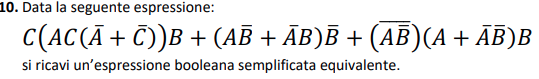
\includegraphics[width=.8\linewidth]{es10_esBoole}
	%\caption{}
	\label{fig:es10esBoole}
\end{figure}

$ \C(\underbrace{\A\C(\negatoA + \negatoC)} _{\underbrace{\A\C\negatoA} _{0} + \underbrace{\A\C\negatoC} _{0}})\B 
+ \underbrace{(\A\negatoB + \negatoA\B)\negatoB} _{\underbrace{\A\negatoBbar\negatoB} _{\A\negatoB} + \underbrace{\negatoA\B\negatoB} _{0}}
+ \underbrace{(\negatoA\overline{\negatoBbar})} _{\negatoA + \B}
+(\underbrace{\A + \negatoA\negatoBbar} _{\A + \negatoB})\B$ \\

$ \Rightarrow 0 \hspace{0.2cm}\text{(Se fossero stati in AND avrebbe azzerato tutto)} + \A\negatoB + 0 + (\negatoA + \B)\underbrace{(\A + \negatoB)\B} _{\A\B + \underbrace{\negatoB\B} _{0}} $ \\

$ \A\negatoB + \underbrace{(\negatoA + \B)\A\B} _{\underbrace{\negatoA\A\B} _{0}
+ \underbrace{\B\A\B} _{\A\B}} $ \\

$ \underbrace{\A\negatoB + \A\B} _{\A(\underbrace{\negatoB + \B} _{1})} $ \\

$ \color{red}\boxed{\normalcolor\A} \hspace{0.3cm}\SOLUZIONE$ \\

% --- ESERCIZIO 11 ALGEBRA DI BOOLE ---

\enlargethispage{18pt}
\begin{figure}[ht]
	%\centering
	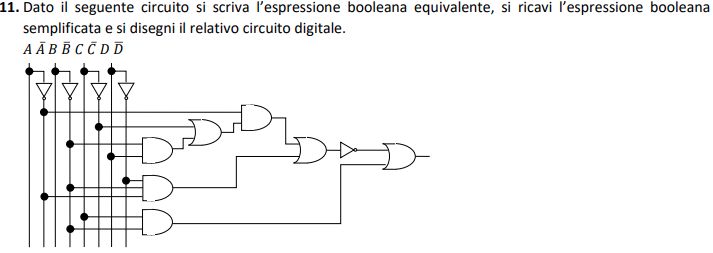
\includegraphics[width=1\linewidth]{es11_esBoole}
	%\caption{}
	\label{fig:es11esBoole}
\end{figure}

$ (\overline{(\underbrace{\negatoB\D + \negatoC)\negatoA} _{\negatoA\negatoBbar\D + \negatoA\negatoCbar} 
	+ \negatoA\negatoBbar\negatoD}) + \negatoB\C$ \\

$ \overline{\negatoA\negatoCbar + \underbrace{\negatoA\negatoBbar\D + \negatoA\negatoBbar\negatoD} _{\negatoA\negatoBbar(\underbrace{\D + \negatoD} _{1})}} + \B\C $ \\

$ \overline{\underbrace{\negatoA\negatoCbar + \negatoA\negatoBbar} _{\demorgan}} + \B\C $ \\

$ \underbrace{(\A + \C)(\A + \B)} _{\A + \B\C} + \B\C $ \\

$ \A + \underbrace{\B\C + \negatoB\C} _{\C(\underbrace{\B + \negatoB} _{1})} $ \\

$ \color{red}\boxed{\normalcolor \A + \C} \hspace{0.3cm}\SOLUZIONE $ \\

\begin{tikzpicture}[label distance=2mm]
	
	\node (x3) at (0,0) {\A};
	\node (x2) at (1,0) {\B};
	\node (x1) at (2,0) {\C};
	\node (x0) at (3,0) {\D};
	
	\node (x4) at (0.5, -0.3) {$ \negatoA $};
	\node (x5) at (1.5, -0.3) {$ \negatoB $};
	\node (x6) at (2.5, -0.3) {$ \negatoC $};
	\node (x7) at (3.5, -0.3) {$ \negatoD $};
	
	\node[not gate US, draw, rotate=-90] at ($(x3)+(0.5,-1)$) (Not3) {};
	\node[not gate US, draw, rotate=-90] at ($(x2)+(0.5,-1)$) (Not2) {};
	\node[not gate US, draw, rotate=-90] at ($(x1)+(0.5,-1)$) (Not1) {};
	\node[not gate US, draw, rotate=-90] at ($(x0)+(0.5,-1)$) (Not0) {};
	
	%\begin{comment}
	\node[or gate US, draw, logic gate inputs=nn] at ($(x0)+(2,-2)$) (Or1) {\text{\logicOR}};
	%\end{comment}
	
	\foreach \i in {3,2,1,0} %aggiungere il 3 se non c'è
	{
		\path (x\i) -- coordinate (punt\i) (x\i |- Not\i.input);
		\draw (punt\i) node[branch] {} -| (Not\i.input);
	}
	%\begin{comment}
	% Allungo le altre linee che non ho usato e anche quelle che ho usato.
	\draw(Not3.output) -- ($(Not3)+(0,-3.35)$);
	\draw(Not2.output) -- ($(Not2)+(0,-3.35)$);
	\draw(Not1.output) -- ($(Not1)+(0,-3.35)$);
	\draw(Not0.output) -- ($(Not0)+(0,-3.35)$);
	
	\draw(x3) -- ($(x3)+(0,-4.35)$);
	\draw(x2) -- ($(x2)+(0,-4.35)$);
	\draw(x1) -- ($(x1)+(0,-4.35)$);
	\draw(x0) -- ($(x0)+(0,-4.35)$);
	
	% OR TRA A E C
	\draw (x3) |- (Or1.input 1);
	\draw (x3 |- Or1.input 1) node[branch] {};
	
	\draw (x1) |- (Or1.input 2);
	\draw (x1 |- Or1.input 2) node[branch] {};
	
	% RIGA FINALE
	\draw (Or1.output) -- ([xshift=0.5cm]Or1.output); %node[above] {$f_1$};
	
	%\end{comment}
\end{tikzpicture}

% --- ESERCIZIO 12 ALGEBRA DI BOOLE ---

\begin{figure}[ht]
	%\centering
	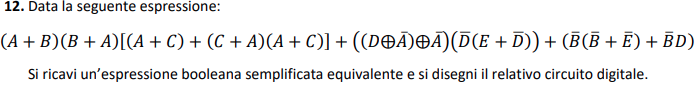
\includegraphics[width=1\linewidth]{es12_esBoole}
	%\caption{}
	\label{fig:es12esBoole}
\end{figure}
%\enlargethispage{60pt}
\begin{equation*}
	\underbrace{(\A + \B)(\B + \A)} _{\A + \B}
	[(\A + \C) + \underbrace{(\C + \A)(\A + \C)} _{\A + \C}] + ((\D\overset{\XOR}{\oplus}\negatoA)\oplus\negatoA)(\underbrace{\negatoD(\E+\negatoD)} _{\negatoD \hspace{0.2cm}\absorption}) + (\underbrace{\negatoB(\negatoB + \negatoE)} _{\negatoB} + \negatoB\D)
\end{equation*}

\begin{equation*}
	(\A + \B)[\underbrace{(\A + \C) + (\A + \C)} _{\A + \C \hspace{0.2cm}\inverse}]
	+ ((\D\oplus\negatoA)\oplus\negatoA)\negatoD + (\underbrace{\negatoB +\negatoB\D} _{\negatoB \hspace{0.2cm}\absorption})
\end{equation*}

\begin{equation*}
	\underbrace{(\A + \B)(\A + \C)} _{\A + \B\C \hspace{0.2cm}\distr} +
	(\underbrace{(\D \oplus \negatoA)\oplus \negatoA} _{\D}) \negatoD + \negatoB
\end{equation*}

\begin{equation*}
	\A + \B\C + \underbrace{\D\negatoD} _{0} + \B
\end{equation*}

\begin{equation*}
	\Rightarrow \A + \underbrace{\B\C + \negatoB} _{\negatoB + \C}
\end{equation*}

\begin{equation*}
	\color{red}\boxed{\normalcolor \A + \negatoB + \C} \hspace{0.3cm}\SOLUZIONE
\end{equation*}


\begin{tikzpicture}[label distance=2mm]
	
	\node (x3) at (0,0) {\A};
	\node (x2) at (1,0) {\B};
	\node (x1) at (2,0) {\C};
	\node (x0) at (3,0) {\D};
	
	\node (x4) at (0.5, -0.3) {$ \negatoA $};
	\node (x5) at (1.5, -0.3) {$ \negatoB $};
	\node (x6) at (2.5, -0.3) {$ \negatoC $};
	\node (x7) at (3.5, -0.3) {$ \negatoD $};
	
	\node[not gate US, draw, rotate=-90] at ($(x3)+(0.5,-1)$) (Not3) {};
	\node[not gate US, draw, rotate=-90] at ($(x2)+(0.5,-1)$) (Not2) {};
	\node[not gate US, draw, rotate=-90] at ($(x1)+(0.5,-1)$) (Not1) {};
	\node[not gate US, draw, rotate=-90] at ($(x0)+(0.5,-1)$) (Not0) {};
	
	%\begin{comment}
	\node[or gate US, draw, logic gate inputs=nnn] at ($(x0)+(2,-2)$) (Or1) {\text{\logicOR}};
	%\end{comment}
	
	\foreach \i in {3,2,1,0} %aggiungere il 3 se non c'è
	{
		\path (x\i) -- coordinate (punt\i) (x\i |- Not\i.input);
		\draw (punt\i) node[branch] {} -| (Not\i.input);
	}
	%\begin{comment}
	% Allungo le altre linee che non ho usato e anche quelle che ho usato.
	\draw(Not3.output) -- ($(Not3)+(0,-3.35)$);
	\draw(Not2.output) -- ($(Not2)+(0,-3.35)$);
	\draw(Not1.output) -- ($(Not1)+(0,-3.35)$);
	\draw(Not0.output) -- ($(Not0)+(0,-3.35)$);
	
	\draw(x3) -- ($(x3)+(0,-4.35)$);
	\draw(x2) -- ($(x2)+(0,-4.35)$);
	\draw(x1) -- ($(x1)+(0,-4.35)$);
	\draw(x0) -- ($(x0)+(0,-4.35)$);
	
	% OR TRA A E B NEGATO E C
	\draw (x3) |- (Or1.input 1);
	\draw (x3 |- Or1.input 1) node[branch] {};
	
	\draw (Not2) |- (Or1.input 2);
	\draw (Not2 |- Or1.input 2) node[branch] {};
	
	\draw (x1) |- (Or1.input 3);
	\draw (x1 |- Or1.input 3) node[branch] {};
	
	% RIGA FINALE
	\draw (Or1.output) -- ([xshift=0.5cm]Or1.output); %node[above] {$f_1$};
	
	%\end{comment}
\end{tikzpicture}

% --- ESERCIZIO 13 ALGEBRA DI BOOLE ---

\begin{figure}[ht]
	%\centering
	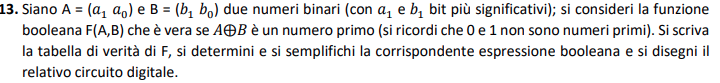
\includegraphics[width=1\linewidth]{es13_esBoole}
	%\caption{}
	\label{fig:es13esBoole}
\end{figure}

\begin{tabular}{|c|c|c|c||c||c||c|}
	\hline
	$a_1$ & $a_0$ & $b_1$ & $b_0$ & $ \A\oplus\B $ & $ F $ &\\
	\hline
	0 & 0 & 0 & 0 & 00 & 0 & \\
	\hline
	0 & 0 & 0 & 1 & 01 & 0 & \\
	\hline
	\tikzmark{startab}0 & 0 & 1 & 0 & 10 & 1 \tikzmark{endab}& $\mathbf{\overline{a_1}\bar{a_0} b_1 \overline{b_0}} $\\
	\hline
	\tikzmark{startbb}0 & 0 & 1 & 1 & 11 & 1 \tikzmark{endbb}& $\mathbf{\overline{a_1}\bar{a_0} b_1 b_0}$\\
	\hline
	0 & 1 & 0 & 0 & 01 & 0 & \\
	\hline
	0 & 1 & 0 & 1 & 00 & 0 & \\
	\hline
	\tikzmark{startcb}0 & 1 & 1 & 0 & 11 & 1 \tikzmark{endcb}& $\mathbf{\overline{a_1}a_0 b_1 \overline{b_0}}$\\
	\hline
	\tikzmark{startdb}0 & 1 & 1 & 1 & 10 & 1 \tikzmark{enddb}& $\mathbf{\overline{a_1}a_0 b_1 b_0}$\\
	\hline
	\tikzmark{starteb}1 & 0 & 0 & 0 & 10 & 1 \tikzmark{endeb}&  $\mathbf{a_1\overline{a_0} \bar{b_1} b_0}$\\
	\hline
	\tikzmark{startfb}1 & 0 & 0 & 1 & 11 & 1 \tikzmark{endfb}& $\mathbf{a_1\overline{a_0} \bar{b_1} b_0}$ \\
	\hline
	1 & 0 & 1 & 0 & 00 & 0 & \\
	\hline
	1 & 0 & 1 & 1 & 01 & 0 & \\
	\hline
	\tikzmark{startgb}1 & 1 & 0 & 0 & 11 & 1 \tikzmark{endgb}& $\mathbf{a_1 a_0 \overline{b_1} \bar{b_0}}$\\
	\hline
	\tikzmark{starthb}1 & 1 & 0 & 1 & 10 & 1 \tikzmark{endhb}& $\mathbf{a_1 a_0 \overline{b_1} b_0}$\\
	\hline
	1 & 1 & 1 & 0 & 01 & 0 & \\
	\hline
	1 & 1 & 1 & 1 & 00 & 0 & \\
	\hline
\end{tabular}

%\begin{comment}
\begin{tikzpicture}[remember picture,overlay]
	\foreach \Val in {ab, bb, cb, db, eb, fb, gb, hb}
	{
		\draw[rounded corners,red,thick]
		([shift={(-0.5\tabcolsep,-0.5ex)}]pic cs:start\Val) 
		rectangle 
		([shift={(0.5\tabcolsep,2ex)}]pic cs:end\Val);
	}
\end{tikzpicture}
%\end{comment}

$ F(a,b,c) = \underbrace{\overline{a_1}\bar{a_0} b_1 \overline{b_0} + \overline{a_1}\bar{a_0} b_1 b_0} 
+ \underbrace{\overline{a_1}a_0 b_1 \overline{b_0} + \overline{a_1}a_0 b_1 b_0} 
+ \underbrace{a_1\overline{a_0} \bar{b_1} b_0 + a_1\overline{a_0} \bar{b_1} b_0}
+ \underbrace{a_1 a_0 \overline{b_1} \bar{b_0} + a_1 a_0 \overline{b_1} b_0}$ \\

$ \color{red}\boxed{\normalcolor \overline{a_1} b_1 + a_1 \overline{b_1}} \hspace{0.3cm}\SOLUZIONE$ \\

$ \color{ForestGreen} a_1 \oplus b_1 $ \\